\documentclass[12pt]{mines-thesis}

%========================================
% Document Setup
%========================================
\DoubleSpacing
\setlength{\parindent}{2em}
\maxtocdepth{subsubsection}

%========================================
% Packages
%========================================
\usepackage{lipsum}
\usepackage{graphicx}
\usepackage{booktabs}
\usepackage{array}
\usepackage{longtable}
\usepackage{natbib}
\usepackage{pdflscape}
\usepackage{everypage}
\usepackage{hyperref}

\urlstyle{same}
\hypersetup{hidelinks}
\graphicspath{{Figures/}}

\begin{document}

%========================================
% Front Matter
%========================================
\autotitle
\title{Example Thesis or Dissertation Title}
\author{Student Name}
\year{2026}
\degree{Doctor of Philosophy}{Program Name}
\advisor{Advisor Name}
% \coadvisor{Co-Advisor Name}
\department{Department or Program Name}
\departmenthead{Department Head Name}

\begin{abstract}
This short abstract demonstrates the front matter structure used by the Mines
thesis template. Replace it with a concise summary of the research problem,
methods, principal results, and conclusions.
\end{abstract}

% Acknowledgments are optional.
\begin{acknowledgment}
This optional page can acknowledge advisors, committee members, collaborators,
funding agencies, family, friends, and others who supported the work.
\end{acknowledgment}

% Dedication is optional. Comment this environment if it is not needed.
\begin{dedication}
\begin{center}
For those who helped make the work possible.
\end{center}
\end{dedication}

\makefrontmatter

%========================================
% Main Body
%========================================
\chapter{Introduction}\label{chap:introduction}

\section{Motivation}

This chapter demonstrates a traditional dissertation chapter. Use separate
files for each chapter so the main file remains short and easy to maintain.
LaTeX handles numbered sections, cross-references, citations, and lists of
figures and tables. For example, Figure~\ref{fig:example-main} and
Table~\ref{tab:example-main} are numbered within Chapter~\ref{chap:introduction}.

\lipsum[2]

\begin{figure}[htbp]
  \centering
  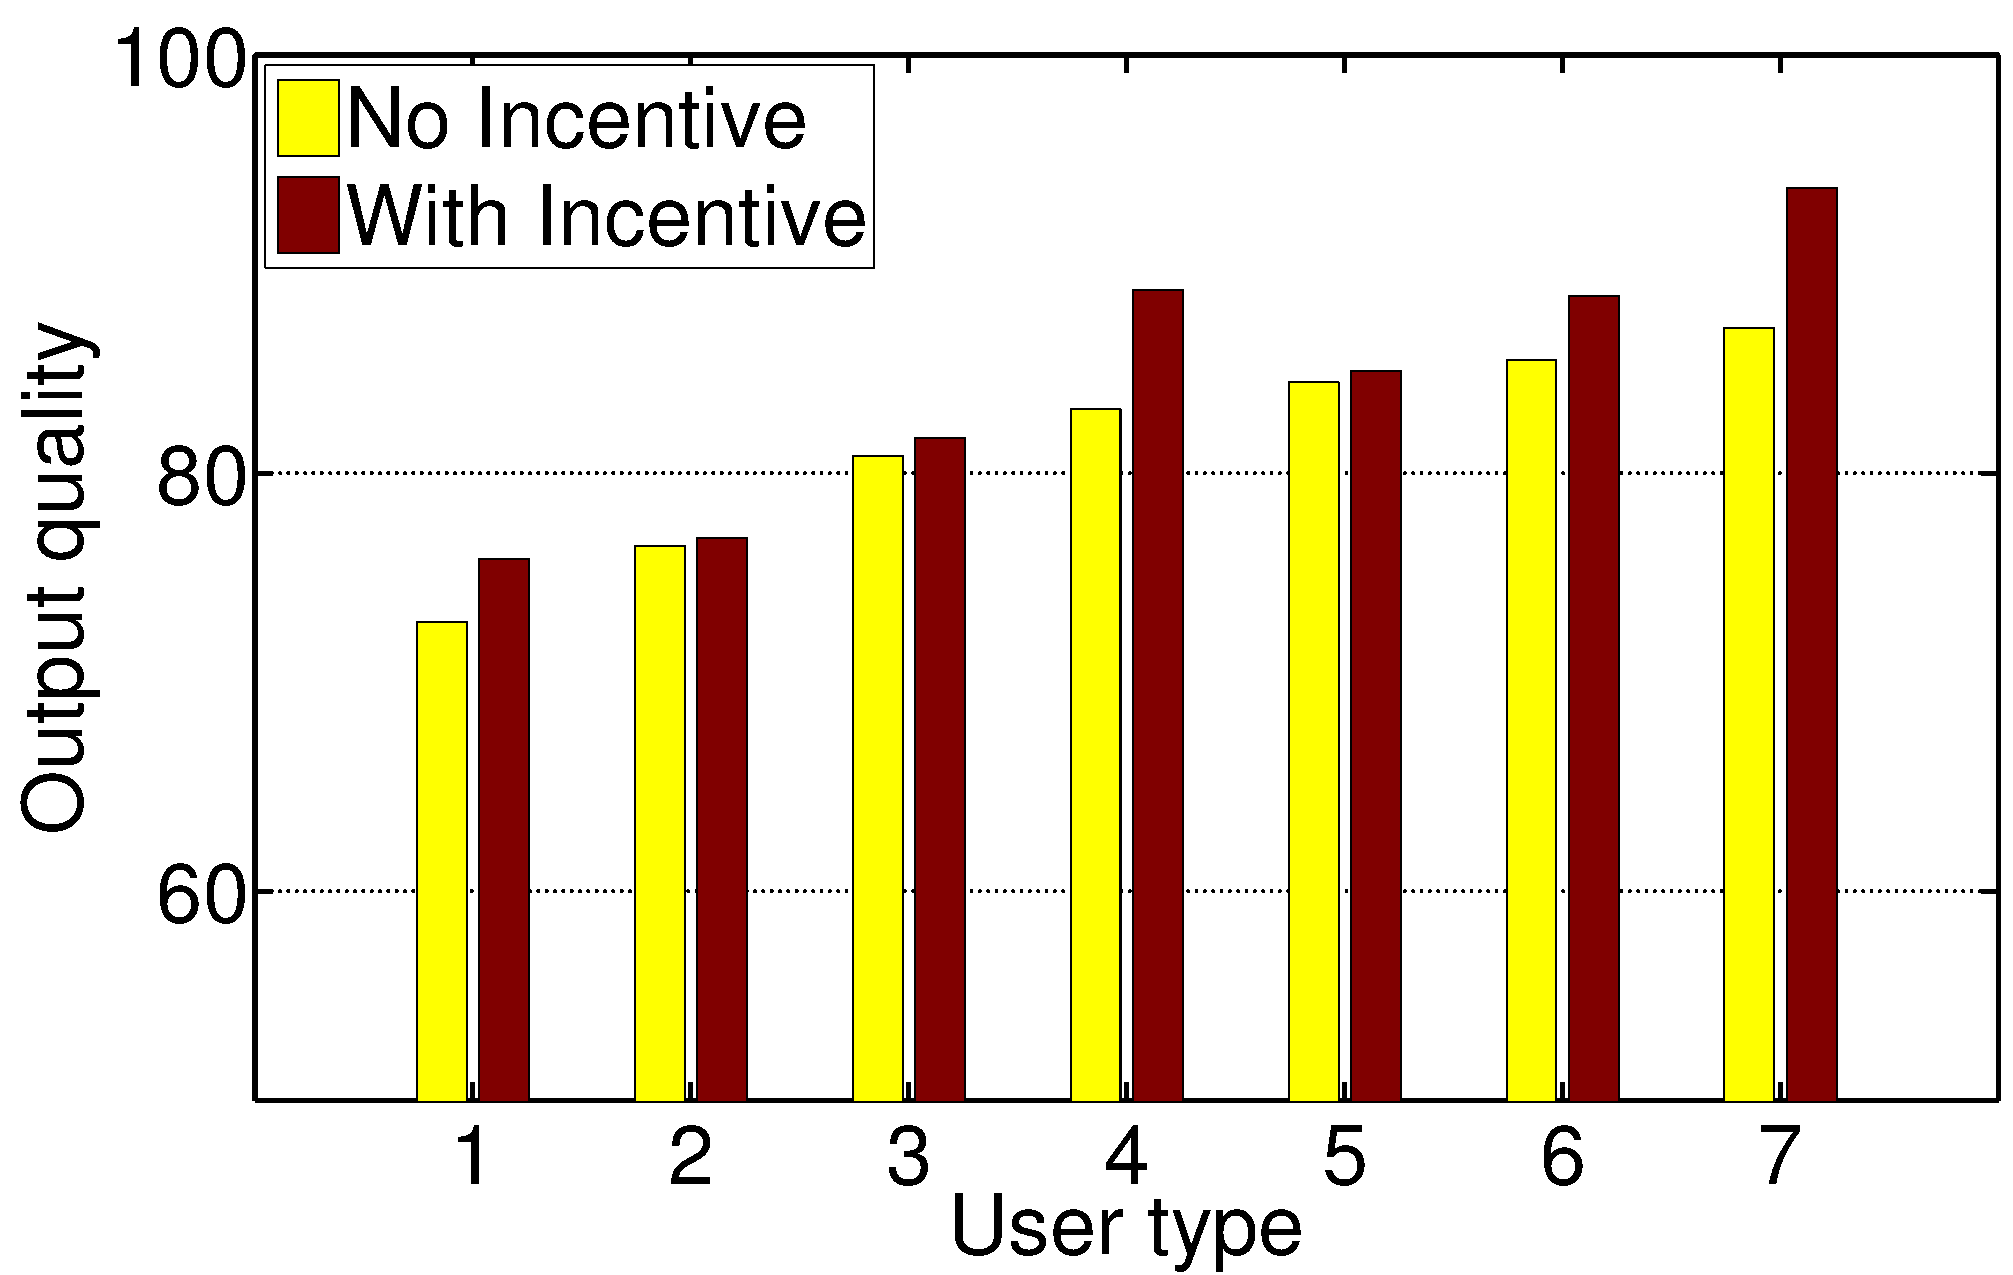
\includegraphics[width=0.75\linewidth]{fig1}
  \caption{Example figure in the main dissertation text.}
  \label{fig:example-main}
\end{figure}

\section{Example Table}

\begin{table}[htbp]
  \caption{Example table using booktabs.}
  \label{tab:example-main}
  \centering
  \begin{tabular}{ll}
    \toprule
    Element & Purpose \\
    \midrule
    Chapters & Main dissertation text \\
    Appendices & Supporting information or supplemental material \\
    References & Bibliography generated from a BibTeX file \\
    \bottomrule
  \end{tabular}
\end{table}

\section{Citations}

This template uses BibTeX and natbib. Parenthetical citations can be written as
\citep{goossens1994latex}; textual citations can be written as
\citet{lamport1994latex}.

\chapter{Example Manuscript Chapter}\label{chap:manuscript}

\reproduceinfo{Modified from a manuscript prepared for journal submission.}

\reproduceabstract
This paragraph demonstrates a manuscript-style chapter abstract. Manuscript
chapters often retain article-like structure inside the dissertation, while the
outer document controls chapter numbering, page numbering, figure numbering,
tables, references, and appendices.

\section{Introduction}

Manuscript-based dissertations often combine several article drafts with a
dissertation introduction, conclusion, and supporting appendices. A practical
workflow is to keep each manuscript chapter in its own \texttt{.tex} file and
include those files from the main dissertation file.

\section{Methods}

Figures and tables in manuscript chapters are numbered by chapter. For example,
Figure~\ref{fig:example-manuscript} appears in Chapter~\ref{chap:manuscript}.

\begin{figure}[htbp]
  \centering
  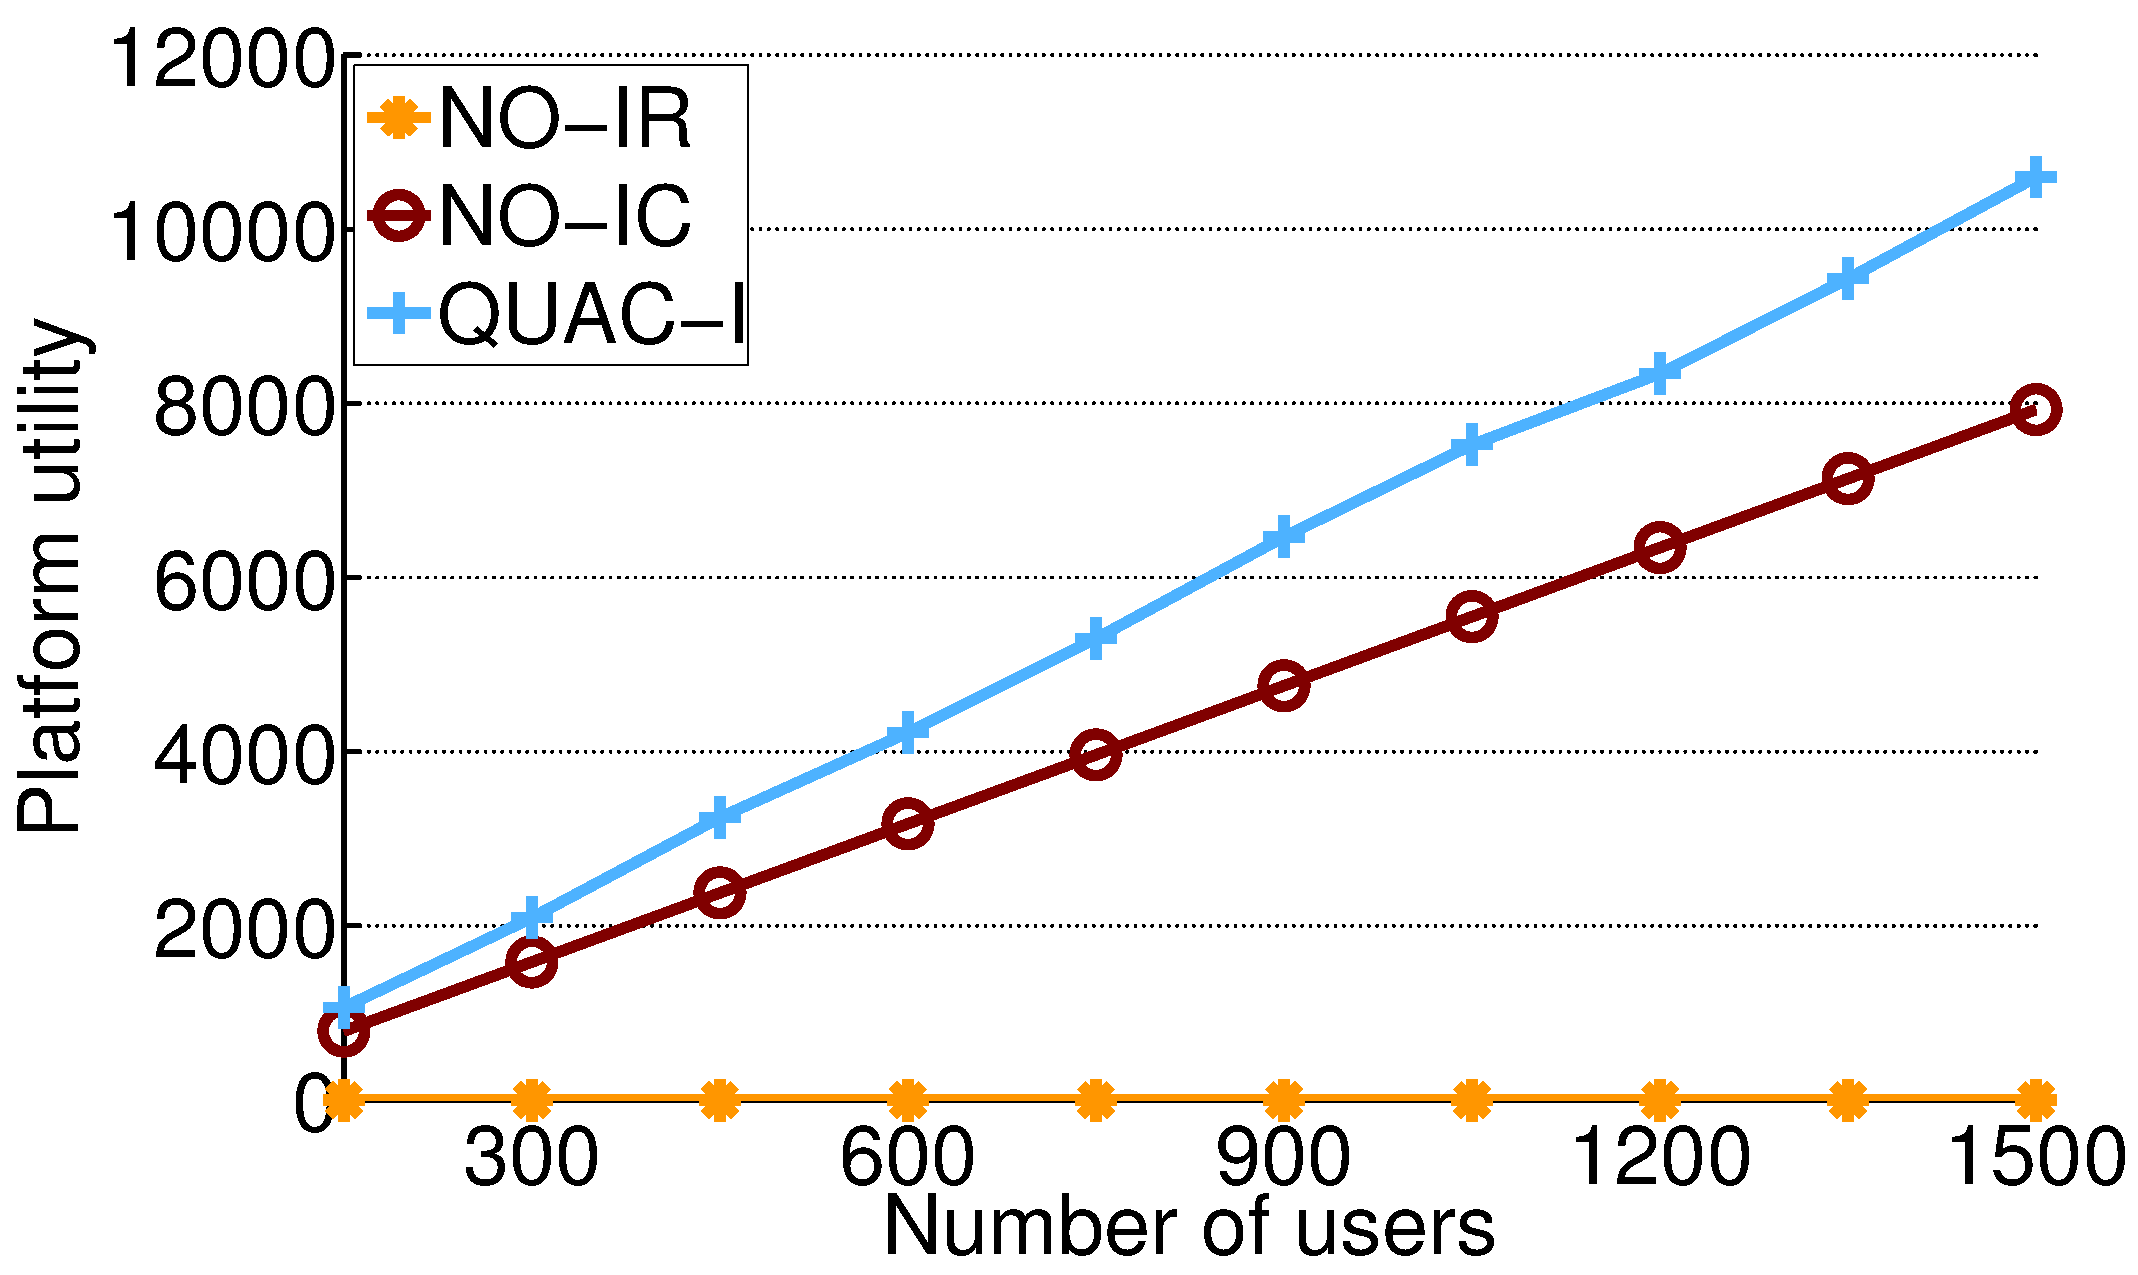
\includegraphics[width=0.6\linewidth]{fig2}
  \caption{Example figure in a manuscript-style chapter.}
  \label{fig:example-manuscript}
\end{figure}

\section{Results}

\lipsum[4]

\section{Discussion}

\lipsum[5]


%========================================
% References
%========================================
\bibliographystyle{apalike}
\bibliography{References/referenceAll}

%========================================
% Appendices
%========================================
\appendix
\chapter{Supporting Information for the Example Manuscript}\label{app:example-si}

Appendices are included after the \verb|\appendix| declaration in the main file.
Figures and tables in appendices should be numbered with appendix letters, such
as Figure~\ref{fig:appendix-example} and Table~\ref{tab:appendix-example}.

\section{Supplemental Figure}

\begin{figure}[htbp]
  \centering
  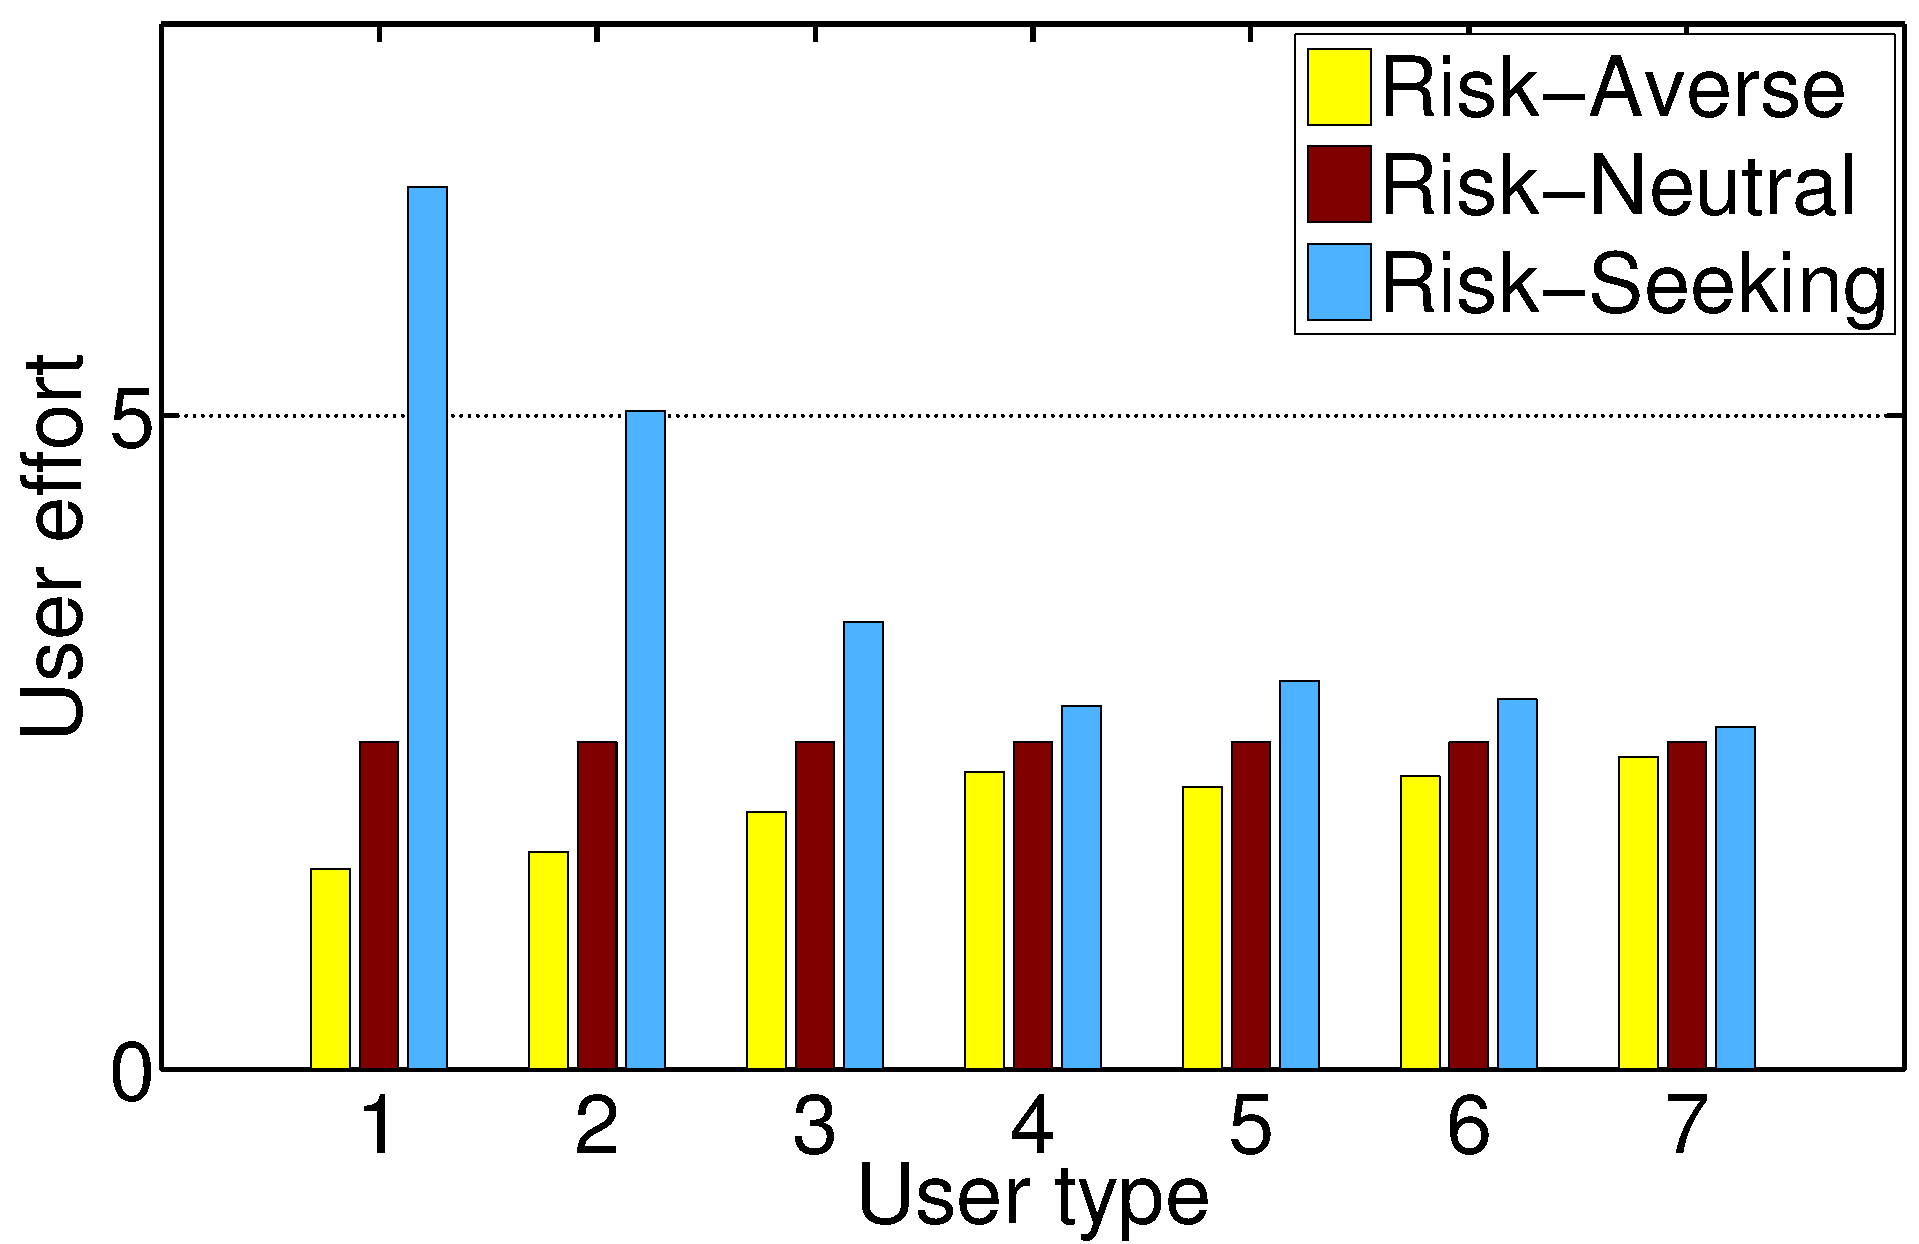
\includegraphics[width=0.75\linewidth]{fig4}
  \caption{Example appendix figure. In the compiled document, this should appear
  as Figure A.1 and should be listed in the List of Figures.}
  \label{fig:appendix-example}
\end{figure}

\section{Supplemental Table}

\begin{table}[htbp]
  \caption{Example appendix table. In the compiled document, this should appear
  as Table A.1 and should be listed in the List of Tables.}
  \label{tab:appendix-example}
  \centering
  \begin{tabular}{ll}
    \toprule
    Item & Notes \\
    \midrule
    Figure numbering & Uses appendix letter and figure number \\
    Table numbering & Uses appendix letter and table number \\
    Cross-references & Use \verb|\ref| or related LaTeX commands \\
    \bottomrule
  \end{tabular}
\end{table}


\end{document}
